\chapter{KD-Trees}\label{chp:kdTrees}

%% \chapterquote{In theory, there is no difference between theory and
%%   practice. But, in practice, there is.}{Jan L. A. van de Snepscheut}

\chapterquote{With todays's fast ray tracers, the difference between a
  ``good'' and a naïvely built kd-tree is often a factor of 2 or
  more.}{Ingo Wald and Vlastimil Havran}



% About KD-trees

Since Arthur Appel described ray tracing four decades ago, several
spatial acceleration structures have been developed to increase the
speed of ray tracers. This chapter will focus on one of the the most
popular acceleration structures, namely the kd-tree.

% Why KD trees

In his ph.d. dissertation \citebook{Havran:PhD}, Vlastimil Havran did
an extensive study of spatial acceleration structures, including
grids, octress and kd-trees. In chapter 3 of the dissertation he
concludes that in most cases the kd-tree will outperform other
well-known acceleration structures.

Since \zhou{}, it has been possible to efficiently construct kd-trees entirely
on the GPU. In the paper they show that their approach even allows ray tracing
dynamic scenes on the GPU, where the kd-tree is reconstructed for each new image
rendered. Building on their approach, I will in \refsection{sec:lowerNodes}
present alternatives to their method for choosing splitting planes. I will also
investigate two different methods for determining when a triangle and a node
overlaps, this is done in \refsection{sec:splittingSchemes}.

Though the different methods and their implementation is presented in this
chapter, the methods will not be evaluated until \refchapter{chp:results}. This
is postponed to allow the introduction of the ray tracers used when evaluating
the quality of the kd-trees in \refchapter{chp:rayTracing}.

% About this Chapter. Start by motivation. Then explain how kd-trees
% are constructed, including different strategies for choosing the
% spliting plane and doing the actual geometry splitting. Then the
% chapter will end with a discussion of how to implement the
% algorithms efficiently on a SIMT architecture.

Before diving into specifics about implementing kd-trees on the GPU, I will
first use the next section to illustrate the recursive kd-tree construction
algorithm in general terms and describe the representation of tree nodes in
memory. The following subsections will then describe different established
algorithms for choosing a splitting plane and how to associate geometry with
child nodes after a split has occured. The latter part of this chapter deals
with converting a single-threaded recursive kd-tree construction algorithm into
a dataparallel algorithm.



\section{Building KD-trees}

A kd-tree is a binary tree that recursively subdivides k-dimensional geometry
into smaller tree nodes. \Refalg{alg:kdTreeCreator} describes a general
recursive kd-tree construction scheme.

\begin{algorithm}
  \caption{Recursive kd-tree constructor}
  \label{alg:kdTreeCreator}
  \begin{algorithmic}
    \PROCEDURE{CreateKdNode}
              {$T$ : Triangle List; $voxel$ : AABB}
              {$node$ : KDNode}
              {\IF{IsLeaf($T, voxel$)}
                  \ASSIGN{$node$}{Leaf(T)}
                \ELSE
                  \COMMENTIT{Determining the splitting plane will be discussed in \refsection{sec:splittingPlane}}
                  \ASSIGN{$plane$}{DeterminePlane($T, voxel$)}
                  \ASSIGN{$(voxel_L, voxel_R)$}{Split($voxel, plane$)}
                  \COMMENTIT{How to associate geometry with a voxel will be the topic of  \refsection{sec:splittingSchemes}}
                  \ASSIGN{$T_L$}{AssociateGeometry($T, voxel_L$)}
                  \ASSIGN{$T_R$}{AssociateGeometry($T, voxel_R$)}
                  \ASSIGN{$node$}{Node($plane$, CreateKdNode($T_L, voxel_L$), CreateKdNode($T_R, voxel_R$))}
                \ENDIF}
  \end{algorithmic}
\end{algorithm}


CreateKdNode takes as arguments a list of triangles and a bounding volume
describing the volume of the node. Usually this bounding volume is an
\textit{axis aligned bounding box}, \textit{AABB}, which is a box whose planes
are aligned with the axes of the coordinate system. An axis aligned bounding
box, $b$, can thus be described by its maximum and minimum values along each
axis and I therefore define it as, $b = \{b_{min}, b_{max}\} \in \{R^3,
R^3\}$. All bounding volumes used in this thesis are axis aligned bounding boxes
and I will therefore use the descriptions bounding volume, bounding box and axis
aligned bounding box interchangeably. CreateKdNode first checks if the
triangles and node's bounding box satisfy the requirements for becoming a leaf
node. If so, then a leaf is produced and the recursion terminates. If not, then
the node's bounding box is divided by a chosen splitting plane, $plane$. How to
determine when to end recursion and choose a splitting plane is the topic of
\refsection{sec:splittingPlane}. Dividing the bounding box produces two new axis
aligned bounding boxes, $voxel_L$ and $voxel_R$. Triangles are then associated
with these new bounding volumes by an association algorithm, which will be
discussed in \refsection{sec:splittingSchemes}. Finally a new node is created
that will contain references to its two children.

An example of an iteration of CreateKdNode can be seen in
\reffig{fig:kdIteration}. The box surrounding the scene is the bounding volume
of the root node. Before the scene has been subdivided by splitting planes, the
root node itself is a leaf node and therefore contains a list of all triangles
associated with it. In \reffig{fig:simpleScene1} a line has been drawn down the
middle of the scene. This line represents a chosen splitting plane and in the
tree's root node it can be seen that the plane splits along the x-axis at $x=4$,
which corrosponds to what is seen in the scene.

\begin{figure}
  \centering \subfloat[A simple scene and it's corrosponding
    kd-tree. The entire scene is contained in the root node.]{
    \begin{tikzpicture}[y=0.5cm, x=0.5cm,font=\sffamily]
      \drawNode{0,0}{8,0}{8,6}{0,6}
      
      % Tris
      \drawTri{0,6}{1,4}{2,5}
      \draw (1,5) node{0};
      \drawTri{4,6}{3,4}{2,5}
      \draw (3,5) node{1};
      \drawTri{4,2}{5,6}{6,4}
      \draw (5,4) node{2};
      \drawTri{8,0}{7,2}{6,1}
      \draw (7,1) node{3};

      %axes
      \draw[->] (0,0) -- coordinate (x axis mid) (9,0);
      \draw[->] (0,0) -- coordinate (y axis mid) (0,7);
      %ticks
      \foreach \x in {0,2,...,9}
     		\draw (\x,1pt) -- (\x,-3pt)
			node[anchor=north] {\x};
    	\foreach \y in {0,2,...,7}
     		\draw (1pt,\y) -- (-3pt,\y) 
     			node[anchor=east] {\y}; 

      \draw (13,3) node [leaf] (0){$\begin{array}{c}0\\\{0, 1, 2, 3\}\end{array}$};
    \end{tikzpicture}
    \label{fig:simpleScene0}
  }

  \subfloat[The same scene as in \reffig{fig:simpleScene0}. The kd-tree has
    split the geometry down the middle and created two new leaf nodes, with
    which the geometry has been associated.]{
    \begin{tikzpicture}[y=0.5cm, x=0.5cm,font=\sffamily]
      \drawNode{0,0}{8,0}{8,6}{0,6}
      
      % Tris
      \drawTri{0,6}{1,4}{2,5}
      \draw (1,5) node{0};
      \drawTri{4,6}{3,4}{2,5}
      \draw (3,5) node{1};
      \drawTri{4,2}{5,6}{6,4}
    \draw (5,4) node{2};
      \drawTri{8,0}{7,2}{6,1}
      \draw (7,1) node{3};

      % Splits
      \draw (4,0) -- (4,6);

      %axes
      \draw[->] (0,0) -- coordinate (x axis mid) (9,0);
      \draw[->] (0,0) -- coordinate (y axis mid) (0,7);
      %ticks
      \foreach \x in {0,2,...,9}
     		\draw (\x,1pt) -- (\x,-3pt)
			node[anchor=north] {\x};
      \foreach \y in {0,2,...,7}
     		\draw (1pt,\y) -- (-3pt,\y) 
     			node[anchor=east] {\y}; 

      \draw (14,4) node [node] (0){$\begin{array}{c}0\\x:4\end{array}$}
        child {node [leaf] (1) {$\begin{array}{c}1\\\{0, 1\}\end{array}$}}
        child {node [leaf] (2) {$\begin{array}{c}2\\\{2, 3\}\end{array}$}};
    \end{tikzpicture}
    \label{fig:simpleScene1}
  }
  \caption{One iteration of the kd-tree construction algorithm.}
  \label{fig:kdIteration}
\end{figure}


\subsection{Tree Representation}\label{sec:treeRepresentation}

Each interior node in a kd-tree must contain three pieces of information.

\begin{itemize}
\item \textit{Split axis} - The axis that an interior node is split
  along.
\item \textit{Split position} - The position of the splitting plane
  along the split axis.
\item \textit{Child references} - Information about how to find the
  node's children.
\end{itemize}

The first two items are pretty straightforward. The choice of axis, x,
y or z, can be stored inside two bits and the position of the splitting
plane should be stored as a floating point number. How an interior
nodes should reference its child nodes, however, is not as
straightforward.

% Left balanced non pointer vs pointers

In general there are two ways a node can reference its child
nodes. The first is through the use of \textit{balanced trees}, where
children of a node can be addressed implicitly without the use of
pointers. The reason for this is that nodes at the same tree level are
placed sequentially in memory and the start address of some tree
level, $l$ is given by $2^l-1$. The left and right child of node $n$
can then be indexed using $2n+1$ and $2n+2$. The parent of a node is
indexed with $\lceil n/2 \rceil - 1$.

% Balanced trees suck, example of partition with high density in one
% side and no triangles in other side. 

Wald et al.\citebook{wald:04:VVH} has the following to say about
balanced trees.

\quotebook{Balancing is optimal only for binary searching, and if all
  nodes have equal access probabilities. Neither of these two
  prerequisites are fulfilled for range queries (such as ray traversal
  and kNN queries), nor for unevenly distributed primitives such as
  photons or triangles.}{wald:04:VVH}

% Choose pointers as that would lead to less memory consumption and it
% places all nodes of the same level in a continues block, making it
% easier to work with them.

To avoid balanced trees we can instead use pointers to reference the
children. This allows for more flexibility when creating the tree. Unfortunately
it also means storing more data per node and in the case of slow memory access
it can cause a memory latency bottleneck. However, when experimenting with
different techniques for creating kd-trees, such as is done in this thesis, the
added flexibility can be a benefit. In \refsection{sec:gpuEmptySpace} we shall
see how this flexibility can be used to add the \textit{Empty Space Maximizing}
optimization, without modifications to the existing kd-tree construction
implementation. This would not have been possible had the tree been balanced.

% Triangle references

The only information that must be stored in a kd-tree's leaf node is how to
reference the triangles associated with it. In this thesis I have choosen to
store a reference to the triangles associated with a leaf as one large list of
indices. I have adopted the convention that all triangle indices associated with
a given leaf must be stored sequentially in memory and a leaf therefore only
needs to contain a reference to its first triangle index and the amount of
triangles it is associated with. Using indices instead of actual triangles makes
it cheaper to perform sorting after a node is split and its triangles associated
with its children. However to simplify the notation and keep the algorithms
simple, in the rest of the thesis I will assume that a leaf has direct access to
the triangles associated with it. When the number of triangles associated with a
node goes below a certain threshold I will switch the representation to an index
and a bit mask. How this will work and the advantages of the bit mask
representation will be explained in \refsection{sec:lowerNodes}.


\subsection{Choosing the Splitting Plane}\label{sec:splittingPlane}

% All the brilliance in KD-tree construction comes down to choosing the
% splitting plane and deciding when to stop.

Looking again at \refalg{alg:kdTreeCreator}, we can see that the brilliance
associated with constructing a high quality kd-tree is knowing where to place
the splitting plane and when to end the recursion and create a leaf.

% Different splitting planes heuristics.

In the following section I present two algorithms that solves this problem and
then I extend them with Empty Space Maximizing, which will improve the quality
of the tree by allowing rays to quickly skip large subtrees and thus find the
geometry that they intersect faster.


\subsubsection{Spatial Median}

% Split at the spatial median.

% Axis to split along can be choosen in a round robin fashion or the
% largest axis can be choosen. (Which initially minimises the surface
% of the children)

A quite simple method for choosing the splitting plane is to place it at the
spatial median of a node's bounding box. There are two ways to choose which
dimensions spatial median to use. A \textit{round robin} fashion can be used,
where the dimensions are cycled every iteration; e.g. when creating the first
node the plane will lie perpendicular to the x-axis, that node's children will
then be split along the y-axis, in the next iteration the nodes will be split
along the z-axis and then the cycle restarts again at the x-axis. Another way of
choosing the dimension is to split along the largest axis of the node's bounding
box. This will be more costly than the round robin approach since more axes must
be analysed, but there is also a higher probability that it will produce trees
of higher quality.

The termination criteria for spatial median splitting is equally as simple as
choosing the splitting plane. If the number of triangles per node falls below a
certain threshold, then recursion stops.

% Refered to as the naïve implementation in Wald07.

This method is refered to as naïve in \citebook{wald:06:NlogN} and rightly so,
since spatial median splitting does not take the distribution of geometry inside
a node's bounding box into account. On \reffig{fig:crapMedian} an example is
given where a node is split in a non-intuitive way. Spatial median splitting
does, however, make up for its suboptimal splitting planes by being quite fast.

 %% and I will therefore use it for creating my kd-trees upper nodes, as
 %% is described in \refsection{sec:upperNodes}.

\begin{figure}
  \centering
  \begin{tikzpicture}[y=0.5cm, x=.5cm,font=\sffamily]
    % AABB
    \draw (0,0) -- (6,0) -- (6,4) -- (0,4) -- (0,0);

    % Tris
    \drawTri{0,0}{2,4}{4,0}
    \drawTri{5,4}{5.5,4}{5,3}
    \drawTri{5,2.5}{5.5,2.5}{5.5,3.5}
    \drawTri{5,2}{6,2}{5.5,0.5}

    % Split
    \draw (3,0) -- (3,4);
    \draw[dashed] (5,0) -- (5,4);

  \end{tikzpicture}

  \vspace{3mm}
  \parbox{5cm}{\caption[A poor split produced by median splitting.]{A poor split
      produced by median splitting. The solid line is a median split. The dashed
      one is a more optimal splitting plane, since it divides the large triangle
      from the small.}\label{fig:crapMedian}}
\end{figure}

\subsubsection{Surface Area Heuristic}\label{sec:SAH}

% SAH assumptions can be seen in Wald07

A far better splitting plane position can be obtained by applying the
\textit{Surface Area Heuristic}, \textit{SAH}. Instead of only considering the
bounding volume surrounding the geometry, SAH considers the entire geometry
associated with a node. In essence SAH computes the \textit{expected cost},
$C_{SAH}$, of traversing a node, $N$, that has been split into the child nodes
$L$ and $R$.

\begin{displaymath}
  C_{SAH}(N \rightarrow \{L, R\}) = C_{trav} + \frac{C_L A_L}{A_N} +
  \frac{C_R A_R}{A_N}
\end{displaymath}

where $C_{trav}$ is the cost of traversing an interior node and is independent
of the splitting plane, $C_L$ is the cost of traversing the left child node and
$C_R$ is the cost of traversing the right child node. $A_n$ is the summed
surface area of the geometry associated with node $n$. Choosing the most optimal
splitting plane amounts to applying SAH to all possible splitting planes and
then choosing the one with lowest cost. Since the above cost evaluation does not
take ray directions into account, SAH assumes that rays are uniformly
distributed, infinite lines.

% Globlly optimal is infeasable for complex scenes and instead a local
% greedy approximation is used.

SAH can also automatically determine when to stop splitting. The cost
of traversing a leaf node is given as

\begin{displaymath}
  C_{leaf}(N) = \|T_N\| C_i
\end{displaymath}

where $\|T_N\|$ is the number of triangles associated with $N$ and $C_i$ is the
cost of testing intersection between a triangle and a ray. SAH's termination
criteria is then $C_{leaf}(N) <= C_{SAH}(N)$, i.e. SAH terminates when the
expected cost of splitting $N$ becomes higher than the cost of keeping $N$ as a
leaf node.

Calculating a globally optimal solution using SAH is infeasable for
complex scenes, as that would require evaluating the cost of all
possible subtrees. A \textit{local greedy approximation} is used
instead, where it is assumed that the created child nodes are
leafs. This assumption simplifies the SAH calculation to

\begin{displaymath}
  C_{SAH}(N \rightarrow \{L, R\}) = C_{trav} + \frac{C_{leaf}(L) A_L}{A_N}
  + \frac{C_{leaf}(R) A_R}{A_N}
\end{displaymath}

The termination criteria can now be simplified into

\begin{displaymath}
  \begin{array}{rl}
    & C_{leaf}(N) <= C_{SAH}(N)\\
    \Updownarrow \\
    & \|T_N\| C_i <= C_{trav} + \frac{C_{leaf}(L) A_L}{A_N} + \frac{C_{leaf}(R)
      A_R}{A_N} \\
    \Updownarrow \\
    & \|T_N\| C_i <= C_{trav} + \frac{\|T_L\| C_i A_L}{A_N} + \frac{\|T_R\| C_i A_R}{A_N}\\
    \Updownarrow \\
    & A_N (\|T_N\| - \frac{C_{trav}}{C_i}) <=  \|T_L\| A_L + \|T_R\| A_R\\
  \end{array}
\end{displaymath}

Deciding on the optimal splitting plane is therefore reduced to finding the
plane with the least weighted area $\|T_L\| A_L + \|T_R\| A_R$ and choosing
appropriate values for the constants $C_{trav}$ and $C_i$ is reduced to
determining $C_{trav}/C_i$.

Inspite of the assumptions made by SAH about ray distribution and that in
practice a local greedy approximation is used, it is still considered one of the
best heuristics and can generally produces trees of the highest quality.

% SAH calculation optimizations include axis round robin and some damn
% paper I can't remember.


\paragraph{Split Candidates}

% To avoid having to test the infinitely many splitting planes
% possible, we instead have to choose sensible planes for SAH.

As mentioned above, the SAH cost needs to be evaluated for \textit{all}
available splitting planes. Since there are infinitely many potential planes
along either axis, some method is needed to distinguish the useful splitting
planes from unimportant ones. The interesting splitting planes are those
finitely many planes, where the geometry association in the resulting left and
right child nodes change. These splitting planes are called \textit{split
  candidates}.

%% and are \textit{tangent planes} to the geometry inside a node's bounding
%% volume. A tangent plane lies perpendicular to a geometric primitives surface
%% and only touches the surface of the triangle without intersecting it.

% Take planes from bounding volumes

The obvious choice of axis aligned split candidates are the 6 planes defined by
a triangle's axis aligned bounding box. These fulfil the requirement for
becoming split candidates, as they represent the exact location where the
geometry association for the left and right side changes. While using the
bounding box' sides is a simple and fast solution, it is not always the most
optimal. The reason for this is that a triangle may not be located entirely
inside a node and therefore its bounding box does not represent the most optimal
split. An example of this can be seen in \reffig{fig:aabbSplit}, where slightly
moving the split candidates given by the sides of the triangle's boudning box
would not change the triangle association in the resulting two leaf nodes.

\begin{figure}
  \centering
  \begin{tikzpicture}[y=0.5cm, x=.5cm,font=\sffamily]

    % AABB
    \drawTri{3,6}{7,2}{6,5}
    \drawAabb{3,2}{7,2}{7,6}{3,6}

    \draw (0,0) -- (6,0) -- (6,5) -- (0,5) -- (0,0);
  \end{tikzpicture}

  \vspace{3mm}
  \parbox{5cm}{\caption[Triangle/Node bounding box intersection.]{An
      example of how the sides of a triangle's bounding box, the
      dashed box, does not represent the most optimal splitting
      planes.}\label{fig:aabbSplit}}
\end{figure}

Another problem with choosing the sides of a triangle's bounding box
as split candidates is that bounding boxes of small nodes may be
completely contained inside the geometry's bounding box. Thus none of
the planes are actually useful split candidates as they can not split
the node, which is demonstrated on \reffig{fig:aabbContained}.

\begin{figure}
  \centering
  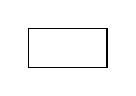
\begin{tikzpicture}[y=0.5cm, x=.5cm,font=\sffamily]

    \drawTri{0,4}{4,0}{3,3}
    \drawAabb{0,0}{4,0}{4,4}{0,4}

    % AABB
    \draw (1,1) -- (3,1) -- (3,2) -- (1,2) -- (1,1);

  \end{tikzpicture}
    
  \vspace{3mm}
  \parbox{5cm}{\caption[A tree node's bounding box contained in a
      triangle's bounding box.]{The kd-tree node's bounding box
      completely contained inside the triangles bounding
      box.}\label{fig:aabbContained}}
\end{figure}

A solution to this is to continuously \textit{clip} the bounding box of the
split geometry to fit the part of the geometry inside the tree nodes bounding
box, which creates optimal split candidates or \textit{perfect split
  condidates}, as demonstrated on \reffig{fig:aabbClipped}.

\begin{figure}
  \centering

  \subfloat[]{
    \begin{tikzpicture}[y=0.5cm, x=.5cm,font=\sffamily]
      
      % AABB
      \drawTri{3,6}{7,2}{6,5}
      \drawAabb{4,3}{6,3}{6,5}{4,5}

      \draw (0,0) -- (6,0) -- (6,5) -- (0,5) -- (0,0);
    \end{tikzpicture}
  }
  \hspace{5mm}
  \subfloat[]{
    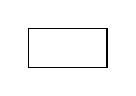
\begin{tikzpicture}[y=0.5cm, x=.5cm,font=\sffamily]

      \drawTri{0,4}{4,0}{3,3}
      \drawAabb{2,1}{2,2}{3,2}{3,1}

      % AABB
      \draw (1,1) -- (3,1) -- (3,2) -- (1,2) -- (1,1);

    \end{tikzpicture}
  }
  \hspace{5mm}
  \subfloat[]{
    \begin{tikzpicture}[y=0.5cm, x=.5cm,font=\sffamily]
      
      \drawTri{0,4}{4,0}{3,3}
      \drawAabb{0,2}{2,2}{2,4}{0,4}
      \drawAabb{2,0}{4,0}{4,3.3}{2,3.3}
      
      % AABB
      \drawNode{-1,0}{2,0}{2,5}{-1,5}
      \drawNode{2,0}{5,0}{5,5}{2,5}

    \end{tikzpicture}
  }

  \vspace{3mm}
  \parbox{10cm}{ \caption[Triangle clipping.]{The triangles' bounding boxes have
      all been clipped to fit the part of the triangle contained in the nodes'
      bounding boxes.}\label{fig:aabbClipped}}
\end{figure}


\subsubsection{Empty Space Maximizing}\label{sec:emptySpace}

An effective optimization to the quality of kd-trees is \textit{Empty Space
  Maximization} and it can be applied to both trees created with Spatial Median
Splitting or SAH. The idea behind the optimization is to cut away large empty
parts of the scene near the top of the tree. This is done by injecting empty
leaf nodes into the tree at interior nodes where the distance from their
parent's bounding box to the associated geometry is above a certain
threshold. The empty nodes will then provide rays traversing the tree with an
early out option, allowing them to skip a large portion of the geometry.

\Reffig{fig:noEmptySpaceExample} shows a simple scene without empty space cut
away and its corrosponding kd-tree. Without Empty Space Maximization the ray
entering the scene from the lower left cornor is forced to perform intersection
tests with every triangle in leaf 1. In contrast the kd-tree in
\reffig{fig:emptySpaceExample} has been created with Empty Space Maximization
enabled and the ray entering the scene now ends up in leaf 4. Leaf 4 is empty
and allows the ray to advance forward while skipping every triangle in leaf 1.

\begin{figure}
  \centering
  \subfloat[A simple scene without empty space cut away.]{
    \begin{tikzpicture}[y=0.5cm, x=.5cm,font=\sffamily]
      
      % AABB
      \draw (0,0) -- (10,0) -- (10,8) -- (0,8) -- (0,0);
      
      % Tris
      \drawTri{9,0}{10,2}{6,3}
      \draw (8.33,1.66) node {5};
      \drawTri{7,8}{7,4}{9,4}
      \draw (7.67,5.33) node {6};
      
      \drawTri{0,8}{0,6}{2,8}
      \draw (0.6,7.3) node {0};
      \drawTri{1,7}{0,6}{2,6}
      \draw (1,6.5) node {1};
      \drawTri{1,7}{3,6}{3,8}
      \draw (2.4,7) node {2};
      \drawTri{5,7}{3,6}{3,8}
      \draw (3.6,7) node {3};
      \drawTri{5,7}{3,6}{6,6}
      \draw (5,6.5) node {4};
      
      % Splits
      \draw (6,0) -- (6,8);
      
      % Ray
      \drawRay{0,0}{3,2}
      
    \end{tikzpicture}
    \label{fig:noEmptySpaceScene}
  }
  \hspace{5mm}
  \subfloat[The tree corrosponding to the scene in \reffig{fig:noEmptySpaceScene}.]{
    \begin{tikzpicture}[y=0.5cm, x=.5cm,font=\sffamily,
        level/.style={sibling distance=20mm/#1}]
      \node [node] {$\begin{array}{c}0\\x:6\end{array}$}
        child {node [leaf] {$\begin{array}{c}1\\\{0,1,2,3,4\}\end{array}$}}
        child {node [leaf] {$\begin{array}{c}2\\\{5, 6\}\end{array}$}};
    \end{tikzpicture}
    \label{fig:noEmptySpaceTree}
  }
  
  \caption[Scene without Empty Space Maximization.]{A kd-tree constructed around
    a simple scene. The kd-tree does not use the Empty Space Maximization
    optimization.}
  \label{fig:noEmptySpaceExample}
\end{figure}

\begin{figure}
  \centering
  \subfloat[The scene from \reffig{fig:noEmptySpaceScene} with empty space cut away.]{
    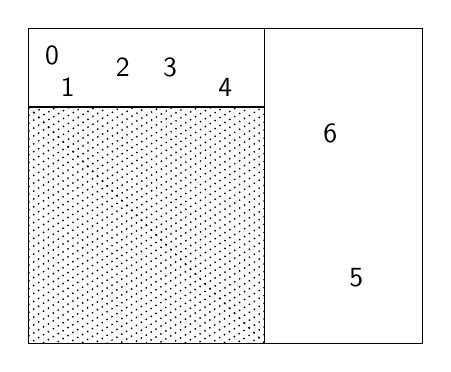
\begin{tikzpicture}[y=0.5cm, x=.5cm,font=\sffamily]
      
      % AABB
      \draw (0,0) -- (10,0) -- (10,8) -- (0,8) -- (0,0);
      
      % Tris
      \drawTri{9,0}{10,2}{6,3}
      \draw (8.33,1.66) node {5};
      \drawTri{7,8}{7,4}{9,4}
      \draw (7.67,5.33) node {6};
      
      \drawTri{0,8}{0,6}{2,8}
      \draw (0.6,7.3) node {0};
      \drawTri{1,7}{0,6}{2,6}
      \draw (1,6.5) node {1};
      \drawTri{1,7}{3,6}{3,8}
      \draw (2.4,7) node {2};
      \drawTri{5,7}{3,6}{3,8}
      \draw (3.6,7) node {3};
      \drawTri{5,7}{3,6}{6,6}
      \draw (5,6.5) node {4};
      
      % Splits
      \draw (6,0) -- (6,8);
      \draw (0,6) -- (6,6);
      
      % Empty space
%      \draw[ball color=gray, color=green, shading=ball,gray] (0,0) -- (0,6) -- (6,6) -- (6,0) -- (0,0);
      \foreach \x in {0,0.2,...,6}
        \draw[line width=0.5pt, dotted] (0, \x) -- (\x, 0);
      \foreach \x in {0,0.2,...,5.8}
        \draw[line width=0.5pt, dotted] (6, \x) -- (\x, 6);
      
      % Ray
      \drawRay{0,0}{6,4}
      
    \end{tikzpicture}
    \label{fig:emptySpaceScene}
  }
  \hspace{5mm}
  \subfloat[The tree from \reffig{fig:noEmptySpaceTree} with the empty space nodes 3 and 4 injected.]{
    \begin{tikzpicture}[y=0.5cm, x=.5cm,font=\sffamily,
        level/.style={sibling distance=40mm/#1}]
      \node [node] {$\begin{array}{c}0\\x:6\end{array}$}
        child {node [node] {$\begin{array}{c}3\\y:6\end{array}$}
            child {node [leaf] {$\begin{array}{c}1\\\{0,1,2,3,4\}\end{array}$}}
            child {node [leaf] {$\begin{array}{c}4\\\emptyset\end{array}$}}
        }
        child {node [leaf] {$\begin{array}{c}2\\\{5, 6\}\end{array}$}};
    \end{tikzpicture}
    \label{fig:emptySpaceTree}
  }
  
  \caption[Empty Space Maximization.]{An example of Empty Space Maximizing. The
    dotted region represents an empty node and allows the ray to leap across it,
    thus skipping intersection tests with the five triangles
    above.}\label{fig:emptySpaceExample}
\end{figure}


Unfortunately, the percentage of a node that should be empty space before it is
cut away is highly scene specific, making this optimization less usefull in the
general case. \zhou{} found that cutting away 25\% or more empty space produced
optimal trees, but instead of simply using their threshold I will test it with
threshold of 15\%, 25\% and 35\% in \refchapter{chp:results}.

% Dynamic empty space threshold, favor early out in the top of the tree.

% huge ray tracing performance improvement in testscene (23% without
% ray tracers doing intersection tests at leaf nodes)

% Implementation is 

\subsection{Triangle/Node Association Schemes}\label{sec:splittingSchemes}

When a splitting plane has been chosen, the interior node's associated triangles
needs to be associated with the child nodes whose bounding box they
overlap. Triangles located entirely in front of the splitting plane are
associated with the left child node and triangles entirely behind are associated
with the right child. The association schemes discussed in this section present
different methods for handling triangles intersected by the splitting plane. The
scheme employed is important in dynamic schemes, on one hand a fast
approximating association scheme may assign triangles to nodes that they do not
necessarily overlap, resulting in larger trees and thus slower ray tracing
times. On the other hand a scheme that rigorously checks every triangle and only
assigns triangles to nodes that they definitely overlap will result in a smaller
tree and faster ray tracing time, but will also incur a performance penalty when
constructing the acceleration structure.



\subsubsection{Triangle Splitting}

% Normally ppl split.

The most common approach when a triangle is intersected by a splitting plane, is
to split the triangle up into new triangles. New triangles produced by triangle
splitting will always be located entirely within the bounding box of the kd-node
they are associated with. When performing triangle splitting there are three
cases to that must be handled, as can be seen in \reffig{fig:splittingCases}.

\begin{figure}
  \centering
  \subfloat[Two vertices to the left of the splitting plane.]{
    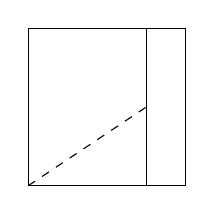
\begin{tikzpicture}[y=0.5cm, x=.5cm,font=\sffamily]
      \draw (0,0) -- (4,0) -- (4,4) -- (0,4) -- (0,0);
      \drawTri{2,4}{0,0}{4,0}
      \draw[dashed] (0,0) -- (3,2);
      \draw (3,0) -- (3,4);
    \end{tikzpicture}
    \label{fig:splittingCase1}
  }
  \hspace{5mm}
  \subfloat[One vertex intersected by the splitting plane.]{
    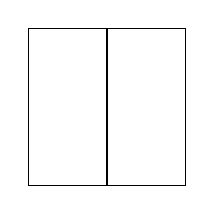
\begin{tikzpicture}[y=0.5cm, x=.5cm,font=\sffamily]
      \draw (0,0) -- (4,0) -- (4,4) -- (0,4) -- (0,0);
      \drawTri{2,4}{0,0}{4,0}
      \draw (2,0) -- (2,4);
    \end{tikzpicture}
    \label{fig:splittingCase2}
  }
  \hspace{5mm}
  \subfloat[Two vertices to the right of the splitting plane.]{
    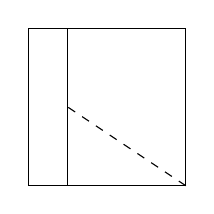
\begin{tikzpicture}[y=0.5cm, x=.5cm,font=\sffamily]
      \draw (0,0) -- (4,0) -- (4,4) -- (0,4) -- (0,0);
      \drawTri{2,4}{0,0}{4,0}
      \draw[dashed] (4,0) -- (1,2);
      \draw (1,0) -- (1,4);
    \end{tikzpicture}
    \label{fig:splittingCase3}
  }

  \vspace{3mm}
  \parbox{10cm}{\caption[The three different triangle splitting
      cases.]{The three different triangle splitting cases. A dashed
      line represents an additional split needed to keep representing
      geometry as triangles.}\label{fig:splittingCases}}
\end{figure}

The first case in \reffig{fig:splittingCase1} illustrates the split when two
vertices are located on the left of the splitting plane and one on the
right. This case is mirrored by \reffig{fig:splittingCase3} where two of the
vertices are located to the right of the splitting plane. In both of these cases
a triangle split will produce three new triangles. The last case in
\reffig{fig:splittingCase2} shows one of the vertices located inside the
splitting plane and splits the triangle perfectly into two new triangles. This
last case however is highly unlikely and in general it can be assumed that a
split triangle always produces three new triangles.


\subsubsection{Triangle/Node Overlap}

\begin{figure}
  \centering
  \subfloat[One split.]{
    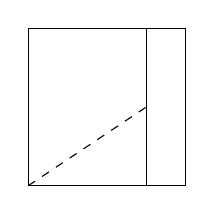
\begin{tikzpicture}[y=0.5cm, x=0.5cm,font=\sffamily]
      \draw (0,0) -- (4,0) -- (4,4) -- (0,4) -- (0,0);
      \drawTri{2,4}{0,0}{4,0}
      \draw[dashed] (0,0) -- (3,2);
      \draw (3,0) -- (3,4);
    \end{tikzpicture}
  }
  \subfloat[Two splits.]{
    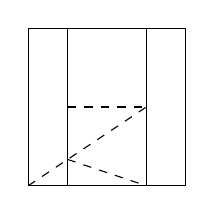
\begin{tikzpicture}[y=0.5cm, x=0.5cm,font=\sffamily]
      \draw (0,0) -- (4,0) -- (4,4) -- (0,4) -- (0,0);

      \drawTri{2,4}{0,0}{4,0}
      
      \draw (1,0) -- (1,4);
      \draw (3,0) -- (3,4);

      \draw[dashed] (1,2) -- (3,2);
      \draw[dashed] (0,0) -- (3,2);
      \draw[dashed] (1,0.667) -- (3,0);
    \end{tikzpicture}
  }
  \subfloat[Three splits.]{
    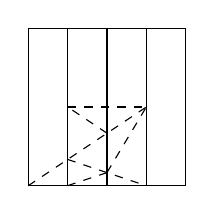
\begin{tikzpicture}[y=0.5cm, x=0.5cm,font=\sffamily]
      \draw (0,0) -- (4,0) -- (4,4) -- (0,4) -- (0,0);
      \drawTri{2,4}{0,0}{4,0}
      
      \draw (1,0) -- (1,4);
      \draw (2,0) -- (2,4);
      \draw (3,0) -- (3,4);

      \draw[dashed] (1,2) -- (3,2);
      \draw[dashed] (0,0) -- (3,2);
      \draw[dashed] (1,0.667) -- (3,0);
      \draw[dashed] (2,0.333) -- (1,0);
      \draw[dashed] (2,0.333) -- (3,2);
      \draw[dashed] (2,1.333) -- (1,2);
    \end{tikzpicture}
  }

  \vspace{3mm}
  \parbox{8cm}{\caption[Excessive splitting of a triangle.]{The triangle splitting
      algorithm performing excessive splits on a triangle.}\label{fig:excessiveSplitting}}
\end{figure}

Since splitting a triangle almost always leads to three new triangles being
created, this can result in excessively many new triangles being created, as
evidenced by \reffig{fig:excessiveSplitting} where the same triangle is split
three times. The problem with excessive splitting is that each new triangle
actually represents the original triangle and on \reffig{fig:excessiveSplitting}
nodes can be seen containing up to 6 triangles, which all represents the exact
same original and are cluttering up the tree with redundant geometry. A more
preferable situation is seen in \reffig{fig:dividing}, where each leaf node only
contains one reference to the original triangle.

\begin{figure}
  \centering
  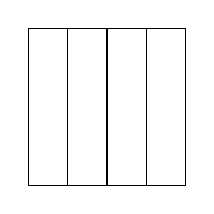
\begin{tikzpicture}[y=0.5cm, x=0.5cm,font=\sffamily]
    \draw (0,0) -- (4,0) -- (4,4) -- (0,4) -- (0,0);
    \drawTri{2,4}{0,0}{4,0}
    
    \draw (1,0) -- (1,4);
    \draw (2,0) -- (2,4);
    \draw (3,0) -- (3,4);
  \end{tikzpicture}
  
  \vspace{3mm}
  \parbox{5cm}{\caption[Dividing a triangle.]{Dividing a triangle among the
      leafs associated with it. Notice that each leaf only contains one
      reference to the original triangle.}\label{fig:dividing}}
\end{figure}

This is the central idea behind performing a \textit{Triangle/Node Overlap}
test. Instead of splitting a triangle by the splitting plane and creating new
triangles, the original triangle is associated with a leaf node if the triangle
and the leaf node's bounding box overlap. How to test this is described in
Möller\citebook{Moller:2005}.

%% Whether or not to associate a triangle and node is decided by performing a
%% \textit{triangle/bounding box overlap} test, as described in
%% Möller\citebook{Moller:2005}. If the triangle overlaps the leaf node's
%% bounding box after the split, then it will be associated with that node,
%% otherwise the triangle will not be a part of that nodes geometry.


\subsubsection{Box Inclusion}\label{sec:boxInclusion}

% Simpler than splitting.

Performing a triangle/bounding box overlap test required for Triangle/Node
Overlap can be a computationally heavy task. A cheaper splitting scheme is to
test if the triangle's axis aligned bounding box, $t$, overlaps with the axis
aligned bounding box of the node, $n$. Performing the overlap test between these
axis aligned bounding boxes is simply

\begin{displaymath}
  \text{overlap}(n,t) = n_{min} < t_{max} \wedge t_{min} < n_{max}
\end{displaymath}

where the infix operator $<: \{R^3, R^3\} \rightarrow bool$ is defined as $n < t
= n.x < t.x \wedge n.y < t.y \wedge n.z < t.z$.

\begin{figure}
  \centering \subfloat[Box Inclusion correctly associates the triangle to both
    nodes.]{
    \begin{tikzpicture}[y=0.5cm, x=.5cm] 
      \drawTri{1,1}{2,4}{4,3}
      \drawAabb{1,1}{1,4}{4,4}{4,1}
      
      \draw (0,0) -- (0,3) -- (3,3) -- (3,0) -- (0,0);
      \draw (3,0) -- (3,3) -- (6,3) -- (6,0) -- (3,0);
    \end{tikzpicture}
  }
  \subfloat[Box Inclusion will incorrectly associate the the triangle with the
    left node.]{
    \begin{tikzpicture}[y=0.5cm, x=.5cm]
      \drawTri{1,2}{2,5}{4,4}
      \drawAabb{1,2}{1,5}{4,5}{4,2}

      \draw (0,0) -- (0,3) -- (3,3) -- (3,0) -- (0,0);
      \draw (3,0) -- (3,3) -- (6,3) -- (6,0) -- (3,0);
    \end{tikzpicture}
    \label{fig:falseBoxInclusion}
  }
  \caption{Box inclusion examples.}
  \label{fig:boxInclusion}
\end{figure}

% Naturally increases amount of \textit{false primitives} in the tree, but is
% very cheap.

\Reffig{fig:boxInclusion} shows two examples of a node being split down the
middle. In both examples the triangle will be associated with both new nodes, as
the triangle's bounding box overlaps both nodes. But in
\reffig{fig:falseBoxInclusion} we clearly see that the triangle itself does not
overlap the right node's bounding box. This illustrates the drawback of only
testing a triangle's bounding box and how box inclusion can produce
\textit{false positives}, where geometric primitives are associated with nodes
they do not overlap. Such false postives will increase the size of the tree and
thus slow down ray tracers. However, Box Inclusion makes up for this by
performing fast node/triangle association, cutting down on the time spent
constructing the tree.



% Also has an increased change of looping during construction in
% combination with a small max lower size. Fx fairy forest loops using
% adjusting bounding box with a max size of 32 primtives in leaf nodes.

% False primitives can then be removed at a later stage at the cost of
% some extra overhead. Or combine with Divide every n'th step for
% optimal sweetness.

% With the added leaf intersection in the ray tracer, extra triangles
% in the leaf nodes become even less important and this method starts
% to shine for dynamic scenes.




\section{Adopting the Algorithms for CUDA}\label{sec:kdTreeImpl}

% Needs to exploit the dataparallel nature of GPU's A GPU needs as many of its
% multiprocessors occupied as possibly for optimal performance.

Having explored the different methods for deciding which splitting plane to use
and how to associate geometry with a node in the kd-tree, it is time to look at
the actual implementation of a kd-tree construction algorithm on the GPU.

The general kd-tree construction method presented in \refalg{alg:kdTreeCreator}
recursively constructs \textit{one} tree node at a time in a
\textit{depth-first} manor. In order to efficiently utilize the GPU, as many of
its multiprocessors as possible must be fully occupied. This means that
\refalg{alg:kdTreeCreator} must be restructured to work on multiple nodes in
parallel. Fortunately this is exactly what \zhou{} did by changing the kd-tree
constructor to work on a list of nodes and recursively create the tree in
\textit{breadth-first} order, as outlined in \refalg{alg:bfsKDTreeCreator}.

\begin{algorithm}
  \caption{BFS recursive kd-tree constructor}
  \label{alg:bfsKDTreeCreator}
  \begin{algorithmic}
    \PROCEDURE{CreateNodes}
              {$activeNodes$ : Node List  \textit{\color{gray}//list of kd-nodes not processed yet}}
              {$nextNodes$ : Node List}
              {\PARALLELFOR{$node$}{$activeNodes$}
                 \IF{IsLeaf($node$)}
                   \ASSIGN{$node$}{Leaf($node$)}
                 \ELSE
                   \COMMENTIT{Determine the splitting plane.}
                   \ASSIGN{$plane$}{DeterminePlane($node$)}
                   \ASSIGN{$(node_L, node_R)$}{Split($node, plane$)}
                   \COMMENTIT{Associate the geometry with a node and add it to the next list.}
                   \ASSIGN{$node_L.geometry$}{AssociateGeometry($node.geometry, node_L$)}
                   \STATE{$nextNodes$.Add($node_L$)}
                   \ASSIGN{$node_R.geometry$}{AssociateGeometry($node.geometry, node_R$)}
                   \STATE{$nextNodes$.Add($node_R$)}
                 \ENDIF
               \ENDFOR}
  \end{algorithmic}
\end{algorithm}

% Creating the KD-tree in BFS will optimize GPU performance at lower tree
% levels, as there would be thousands of nodes created at the same time.

At the bottom levels, where thousands of nodes are created in parallel,
breadth-first creation allows full utilization of the GPU. But for the upper
levels of the tree this approach will still not fully exploit the graphics
hardware, as only a couple of nodes are active per iteration, leaving the
multiprocessors underutilized.

To remedy this the tree construction will be split into two phases, an upper and
a lower phase. A node is said to belong to the upper part of the tree if the
number of triangles associated with it is above a given threshold. In this
thesis I will be using the thresholds 32 and 64. During the upper tree creation
phase, the choice of splitting plane is parallelized over all geometric
primitives, of which there can be hundreds of thousands. When creating the lower
tree, there will be thousands of nodes and computations can effectively be
structured as in \refalg{alg:bfsKDTreeCreator}.

% The structure of the rest of the chapter.

The overall construction of the tree is presented in
\refalg{alg:constructKDTree}. First the axis aligned bounding box for each
triangle is precomputed. These are used to effectively compute the bounding
boxes of nodes and for box inclusion, if that association scheme is used. Then
the upper part of the tree is constructed iteratively until there are no more
new nodes to process. How this is achieved is the topic of
\refsection{sec:upperNodes}. Once the upper part of the tree is constructed, the
leaf nodes are processed to prepare for the lower tree construction phase. The
lower part of the tree is then iteratively constructed and
\refsection{sec:lowerNodes} details three different algorithms that produces
lower trees with varying construction speed and quality.

\begin{algorithm}
  \caption{Construct kd-tree}
  \label{alg:constructKDTree}
  \begin{algorithmic}
    \PROCEDURE{ConstructKDTree}
              {$Triangles$ : Triangle List}
              {$root$ : Node}{
                \PARALLELFOR{$t$}{$Triangles$}
                  \STATE{Compute axis aligned bounding box for $t$.}
                \ENDFOR
                \STATE{}
                \DECLARE{$activeNodes, leafs, nextNodes$}{Node List}
                \COMMENTIT{Upper node construction phase.}
                \STATE{$activeNodes$.Add($rootNode$)}
                \WHILE{$activeNodes$.NotEmpty}
                  \STATE{$nextNodes$.Clear}
                  \ASSIGN{$(newLeafs, nextNodes)$}{CreateUpperNodes($activeNodes$)}
                  \STATE{$leafs$.Append$(newLeafs)$}
                  \STATE{swap($activeNodes$, $nextNodes$)}
                \ENDWHILE
                \STATE{}
                \COMMENTIT{Lower node construction phase.}
                \STATE{PreprocessLowerNodes($leafs$)}
                \STATE{CreateLowerNodes($leafs$, $activeNodes$)}
                \WHILE{$activeNodes$.NotEmpty}
                  \STATE{$nextNodes$.Clear}
                  \ASSIGN{$nextNodes$}{CreateLowerNodes($activeNodes$)}
                  \STATE{swap($activeNodes$, $nextNodes$)}
                \ENDWHILE
              }
  \end{algorithmic}
\end{algorithm}

\subsection{Upper Tree Creation}\label{sec:upperNodes}

% At upper tree level nodes exploit data parallelism by parallelizing the cost
% computation over triangles.

At the uppermost levels of the kd-tree there will not be many nodes over which
the computation can be parallelized. But each node can be associated with
thousands of geometric primitives and parallelizing the choice of splitting
plane across the geometry will utilize the GPU effectively.

% SAH assumes that each split results in two leaf nodes, which is practically
% always wrong at high level nodes, therefore \zhou{} suggests splitting along
% the spatial median of the nodes longest axis.

The issue is then which algorithm to use when choosing the splitting plane. The
Surface Area Heuristic provides an algorithm that easily can be parallelized
over the geometry. Each triangle would then be responsible for computing the
expected cost of splitting a node with its 6 bounding box planes and afterwards
the best possible plane could be reduced with the method described in
\refsection{sec:reduce}. Unfortunately there can be hundreds of thousand of
triangles associated with the tree's upper nodes, so comparing a split candidate
to all of them becomes computationally heavy. SAH also assumes that the created
children will be leaf nodes in the final tree and therefore that their cost can
be computed using $C_{leaf}$, which is almost never true at the top of the
tree. This makes SAH an undesirable algorithm for choosing splitting planes for
the upper tree, since we need to be able to decide on which splitting plane to
use fast to accomodate dynamic scenes. Instead \zhou{} proposes to use spatial
median splitting with Empty Space Maximization. Parallizing the splitting plane
decision over the geometry then becomes reducing an axis aligned bounding box
from a node's associated triangles, again as described in
\refsection{sec:reduce}, and then each node can use that bounding box to decide
where to place its splitting plane.

To associate triangles and nodes in the upper parts of the tree, both schemes
described in \refsection{sec:splittingSchemes} can be employed. As with the
splitting plane decision, the triangle/node association scheme will be
parallelized over all triangles. Since I have made the assumption that all
triangles associated with a node must be placed sequentially in memory, the
triangles need to be sorted after the triangle/node association has been
determined. To parallelize this sorting over all triangels, I again make use of
the scan primitive described in \refsection{sec:GPUprims}. Since a triangle can
be associated with both child nodes, the left-right sorting in
\refsection{sec:GPUprims} is not directly applicable. Instead I will be using a
variant where the prefix-sum calculation is applied to a list of size $2 \cdot
\|triangles\|$. In the first half of the list I will then use 0's and 1's to
represent whether the $t$'th triangle overlapped its current node's left
child. The last half of the list does the same but for the right
child. Computing the prefix-sum of this list then yields the addresses,
$associateAddr$, where the triangles should be copied to. Below is an example of
this

\begin{displaymath}
  \begin{array}{r c c c c c c c c c c c c c}
    triangles: & [t_0 & t_1 & t_2 & t_3 & t_4 & t_5] & \color{lightgray}[t_0 & \color{lightgray}t_1 & \color{lightgray}t_2 & \color{lightgray}t_3 & \color{lightgray}t_4 & \color{lightgray}t_5]\\
    left/right: & [1 & 1 & 0 & 1 & 1 & 0 & 1 & 0 & 1 & 0 & 0 & 1]\\
    associateAddr: & [0 & 1 & 2 & 2 & 3 & 4 & 4 & 5 & 5 & 6 & 6 & 6 & 7]\\
    sorted: & [t_0 & t_1 & t_3 & t_4 & t_0 & t_2 & t_5]
  \end{array}
\end{displaymath}

where the $triangles$ list is duplicated to easily show the association between
the entries in $left/right$ and the triangles. With the $left/right$ and
$associateAddr$ lists it is possible to parallelize the triangle sorting
effectively over all triangles using the algorithm in \refalg{alg:triangleSort}.

\begin{algorithm}
  \caption{Parallel triangle sorting.}
  \label{alg:triangleSort}
  \begin{algorithmic}
    \PROCEDURE{TriangleSort}
              {$triangles$ : Triangle List, $left/right$ : Bit List, $associateAddr$ : Integer List}
              {$sorted$ : Triangle List}
              {\DECLARE{$sorted$}{Triangle List}
                \PARALLELFOR{$t$}{$triangles$}
                \IF{$left/right$[$t$]}
                  \ASSIGN{$addr$}{$associateAddr$[$t$]}
                  \ASSIGN{$sorted$[$addr$]}{$t$}
                \ENDIF
                \IF{$left/right$[$t + \|triangles\|$]}
                  \ASSIGN{$addr$}{$associateAddr$[$t + \|triangles\|$]}
                  \ASSIGN{$sorted$[$addr$]}{$t$}
                \ENDIF
               \ENDFOR}
  \end{algorithmic}
\end{algorithm}

% Explain the overall strcuture, how the last n nodes are active
% nodes?

\begin{figure}
  \centering
  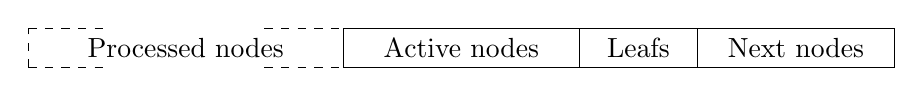
\begin{tikzpicture}[y=0.5cm, x=0.5cm]
    \draw[dashed] (0,1) -- (2,1);
    \draw[dashed] (0,0) -- (0,1);
    \draw[dashed] (0,0) -- (2,0);
    \draw (4,0.5) node {Processed nodes};
    \draw[dashed] (6,1) -- (8,1);
    \draw[dashed] (6,0) -- (8,0);
    \draw (8,1) -- (8,0);

    \draw (8,1) -- (22,1);
    \draw (8,0) -- (22,0);

    \draw (11,0.5) node {Active nodes};
    \draw (14,1) -- (14,0);

    \draw (15.5,0.5) node {Leafs};
    \draw (17,1) -- (17,0);

    \draw (19.5,0.5) node {Next nodes};
    \draw (22,1) -- (22,0);

  \end{tikzpicture}
  \caption{The structure of the kd-trees nodes in memory.}
  \label{fig:nodeStructure}
\end{figure}

\fixme{Place this somewhere else?}

Like the triangles, the nodes themselves are placed in one large array with the
structure shown in \reffig{fig:nodeStructure}. The already processed nodes are
placed in one sequential chunk from index 0. The currently active nodes are
located right after them. The child nodes created by
\refalg{alg:kdUpperNodeCreator} are then placed after the active nodes, with the
leaf nodes to the left and next set of active nodes to the right. This preserves
the invariant that the $n$ currently active nodes, if any, are always the $n$
last nodes in the array after an iteration of the construction algorithm. This
is a desirable property as it means I do not need to maintain a list of indices
to active nodes, but can instead describe the list $activeNodes$ by a range and
an index into the node list. This also improves coalescence when subsequent
threads can access nodes sequentially.


\begin{algorithm}
  \caption{KD-Tree upper node creator}
  \label{alg:kdUpperNodeCreator}
  \begin{algorithmic}
    \PROCEDURE{CreateUpperNodes}
               {\VAR{activeNodes} : Node List}
               {\VAR{leafs,nextNodes} : Node List}{
                 \COMMENTIT{First split all triangles into segments.}
                 \DECLARE{$segmentList$}{List}
                 \PARALLELFOR{$node$}{$activeNodes$}
                   \STATE{Split all triangles contained in $node$ into
                     fixed sized segments and store those in $segmentList$.}
                 \ENDFOR
                 \STATE{}
                 \COMMENTIT{Then compute each triangles bounding box
                   using reduction as described in
                   \refsection{sec:reduce}.}
                 \PARALLELFOR{$segment$}{$segmentList$}
                   \STATE{Compute the bounding box of the triangles in
                     each segment.}
                 \ENDFOR
                 \STATE{Use segmented reduction as described in
                   \zhou{} to compute each nodes bounding box.}
                 \PARALLELFOR{$node$}{$activeNodes$}
                   \STATE{Split $node$ along its spatial median.}
                 \ENDFOR

                 \STATE{}
                 \COMMENTIT{Perform Empty Space Maximization.}
                 \COMMENTIT{See \refalg{alg:emptySpaceMaximizing}.}
                 \STATE{...}
                 \STATE{}

                 \COMMENTIT{Compute the addresses to sort the
                   triangles to by comparing them to the splitting
                   plane.}
                 \DECLARE{$associateSide, associateAddr$}{List}
                 \PARALLELFOR{$segment$}{$segmentList$}
                   \PARALLELFOR{$triangle$}{$segment.triangles$}
                     \ASSIGN{$associateSide[triangle.id]$}{AssociateLeft($segment.node$, $triangle$)}
                     \ASSIGN{$associateSide[triangle.id + \|triangles\|]$}{AssociateRight($segment.node$, $triangle$)}
                   \ENDFOR
                 \ENDFOR
                 \ASSIGN{$associateAddr$}{\textbf{Prefix-Sum}($associateSide$)}
                 \COMMENTIT{Sort the triangles.}
                 \ASSIGN{$triangles$}{TriangleSort$(triangles, associateSide, associateAddr)$}
                 %% \PARALLELFOR{$segment$}{$segmentList$}
                 %%   \PARALLELFOR{$triangle$}{$segment.triangles$}
                 %%     \STATE{Sort the triangles to have triangles
                 %%       associated with the same node placed
                 %%       sequentially.}
                 %%   \ENDFOR
                 %% \ENDFOR

                 \STATE{}

                 \COMMENTIT{Split nodes.}
                 \PARALLELFOR{$node$}{$activeList$}
                   \STATE{Split the nodes into child
                     nodes. $associateSide$ and $associateAddr$ is
                     used to directly calculate the child nodes
                     triangle index and range.}
                   \COMMENTIT{Sort child nodes into the leaf and nextNodes
                     list. This is achieved just like the example from
                     \refsection{sec:GPUprims}.}

                   \IF{$node.child$.size < $threshold$}
                     \STATE{$leaf$.Add($node.child$)}
                   \ELSE
                     \STATE{$nextNodes$.Add($node.child$)}
                   \ENDIF
                 \ENDFOR
  }
  \end{algorithmic}
\end{algorithm}

% Go over the algorithm

The algorithm for constructing the upper parts of the kd-tree can be
seen in \refalg{alg:kdUpperNodeCreator}. It takes a list of non
processed nodes, $activeNodes$ as input and returns a list of leaf
nodes, $leafs$, and a list of new nodes, $nextNodes$, that needs to be
processed in the next iteration.


% Use GPU for computations and let CPU handle minor book keeping.

The first thing that \refalg{alg:kdUpperNodeCreator} does is split the triangles
associated with each active node into fixed-size segments. This may seem odd at
first, but recall that the upper nodes are split along the spatial median, that
finding the spatial median means computing a tight bounding box around the
geometry associated with a node, and that to do this we need to apply the
reduction described in \refsection{sec:reduce}. Generally having fixed-size
segments will also make it easier to choose a kernels block size, so that each
segment is processed by one block. A segment contains information about which
triangles it contains, which node its triangles are associated with and, incase
there are not enough triangles to fill it, it also stores how many triangles it
actually contains. The reduction kernel can use this information to pad the data
loaded into shared memory with identity elements.

After having segmented the triangles, the bounding boxes of teh individual
segments can be computed as shown in \refsection{sec:reduce} by using the
operators \textbf{min} and \textbf{max} with their identity elements. Then
performing a segmented reduction on the result, as described in Algorithm 3 in
\zhou, will compute a tight bounding box for each node in activeList. A kernel
working on all active nodes can then use this bounding box to place the nodes
splitting planes along their spatial median.

With the splitting plane determined for each node, the triangles will be able to
determine their triangle/node association with the nodes children and sort
themselves into a new list as described above.

%% Instead of reducing the sizes of child nodes, as done in \zhou{} I propose a
%% method for calculating them directly. This leads to lots of uncoalesced
%% lookups, so argue if the GPU is able to properly hide these.

Lastly the nodes in $activeList$ are split into their child nodes in
parallel. For node $n$, the values in $associateAddr$ can be used to calculate
the triangle index and range of the child nodes, $left$ and $right$, as seen in
\refalg{alg:childIndices}. The idea behind \refalg{alg:childIndices} is that
using the triangle index of the parent nodes we are able to extract the triangle
index of its left and right child nodes. Then by adding the number of triangles
in the parent node to its index, we can lookup the starting index of the next
child node's triangles. Subtracting these two values yields the range of
triangles spanned by a child node.

\begin{algorithm}
  \caption{Compute child node triangle index and range}
  \label{alg:childIndices}
  \begin{algorithmic}
    \PROCEDURE{ChildTriangleInformation}
              {$parent, left, right$: Node, $associateAddr$ : List}
              {$left$ : Node, $right$ : Node}{
                \ASSIGN{$left.triangleIndex$}{$associateAddr[parent.triangleIndex]$}
                \ASSIGN{$leftEndAddr$}{$associateAddr[parent.triangleIndex + parent.triangleRange]$}
                \ASSIGN{$left.triangleIndex$}{$leftEndAddr - left.triangleIndex$}
                \ASSIGN{$right.triangleIndex$}{$associateAddr[parent.triangleIndex + \|triangles\|]$}
                \ASSIGN{$rightEndAddr$}{$associateAddr[parent.triangleIndex + parent.triangleRange]$}
                \ASSIGN{$right.triangleIndex$}{$rightEndAddr - right.triangleIndex$}
              }
  \end{algorithmic}
\end{algorithm}



% Building the upper nodes mostly consist of moving data around, and
% not necessarily in a coalesced fashion. This makes it hard to hide
% the latency and will impact performance.

% Argue it can be done in O ( N log N )



\subsubsection{Adding Empty Space Maximizing}\label{sec:gpuEmptySpace}

% Plugable solution, add the new nodes after the ones in nextlist.

To experiment with the Empty Space Maximization optimization it needs to be
implemented as a solution that can be turned on and off at will. This has been
achieved with the design found in \refalg{alg:emptySpaceMaximizing}, which
injects new nodes created by Empty Space Maximizing into the tree. In order to
perform Empty Space Maximizing a \textit{loose bounding box} needs to be
propagated down the tree. A loose bounding box is computed by splitting a
parents bounding box with its splitting plane. Since the geometry inside a child
might not touch all sides of a parents bounding box, the loose bounding box
provides a loose upper bound on the geometry.

\begin{algorithm}
  \caption{Calculate Empty Space Maximization}
  \label{alg:emptySpaceMaximizing}
  \begin{algorithmic}
    \PROCEDURE{CreateUpperNodes}
               {\VAR{activeNodes} : Node List}
               {\VAR{leafs,nextNodes} : Node List}{

                 \COMMENTIT{First split all triangles into segments.}
                 \STATE{...}
                 \COMMENTIT{Then compute each triangles bounding box
                   using reduction as described in
                   \refsection{sec:reduce}.}
                 \STATE{...}

                 \STATE{}
                 \COMMENTIT{Perform Empty Space Maximization.}
                 \IF{$performEmptySpaceMaximization$}
                 \DECLARE{$emptySplitNodes, emptyAddr$}{List}
                 \DECLARE{$emptySides$}{Plane List}
                 \PARALLELFOR{$node$}{$activeList$}
                 \ASSIGN{$emptySplits[i]$}{$0$}
                   \FOREACH{$side$}{$node.boundingBox$}
                     \IF{$node$ has more than $C_e$ empty space on $side$}
                       \ASSIGN{$emptySplitNodes[i]$}{$emptySplitNodes[i] + 2$}
                       \STATE{$emptySides[node]$.Add($side$)}
                     \ENDIF
                   \ENDFOR
                 \ENDFOR
                 \ASSIGN{$emptyAddr$}{\textbf{Prefix-Sum}($emptySplitNodes$)}
                 \PARALLELFOR{$node$}{$activeList$}
                   \STATE{Cut of empty space of sides in $emptySides$ and place
                     new nodes sequentially at addresses specified in
                     $emptyAddr$. Then rewire parent nodes to point to new
                     nodes.}
                 \ENDFOR
                 \ENDIF

                 \STATE{}
                 \COMMENTIT{Compute the addresses to move the
                   triangles to by comparing them to the splitting
                   plane.}
                 \STATE{...}
                 \COMMENTIT{Move the triangles.}
                 \STATE{...}

                 \COMMENTIT{Split nodes.}
                 \STATE{...}
  }
  \end{algorithmic}
\end{algorithm}

% Explain

The algorithm for performing Empty Space Maximization is inserted right after
computing the nodes' tight bounding boxes and before the new child nodes are
created. Whether or not Empty Space Maximization should be performed on any of
the nodes in $activeNodes$ is then checked in parallel for all nodes. The sides
of a node's bounding box is checked sequentially to see if the empty space
between the loose and the tight bounding box is above a certain threshold, which
means that the empty space should be cut away. These sides are added to the list
$emptySides$, which will be used later when the nodes are split. Each such split
results in two new nodes, one node that refers to the empty space and one node
injected between the parent node and its child node in active list. This
injection is depicted in \vreffig{fig:noEmptySpaceExample} and
\vreffig{fig:emptySpaceExample}. The number of new nodes created per node in
$activeList$ by performing Empty Space maximization is stored in
$emptySplitNodes$.

Once the sides that should have empty space cut away has been determined, where
to place the nodes created by these splits are computed by calculating the
prefix-sum of $emptySplitNodes$. Empty Space Maximization nodes are injected
into to the list of nodes shown in \reffig{fig:nodeStructure} as described on
\reffig{fig:emptyNodeStructure}, which again preserves the invariant that the
next batch of active nodes are located at the end of the list. The arrows in
\reffig{fig:emptyNodeStructure} symbolize the parent$\rightarrow$child
relationship and very accuratly show how the new nodes are injected into the
tree.

\begin{figure}
  \centering
  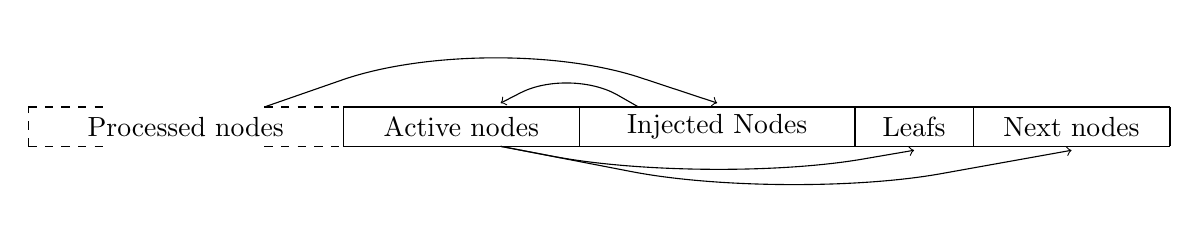
\begin{tikzpicture}[y=0.5cm, x=0.5cm]
    \draw[dashed] (0,1) -- (2,1);
    \draw[dashed] (0,0) -- (0,1);
    \draw[dashed] (0,0) -- (2,0);
    \draw (4,0.5) node {Processed nodes};
    \draw[dashed] (6,1) -- (8,1);
    \draw[dashed] (6,0) -- (8,0);
    \draw (8,1) -- (8,0);

    \draw (8,1) -- (29,1);
    \draw (8,0) -- (29,0);

    \draw (11,0.5) node {Active nodes};
    \draw (14,1) -- (14,0);

    \draw (17.5,0.5) node {Injected Nodes};
    \draw (21,1) -- (21,0);

    \draw (22.5,0.5) node {Leafs};
    \draw (24,1) -- (24,0);

    \draw (26.5,0.5) node {Next nodes};
    \draw (29,1) -- (29,0);

    \draw[rounded corners=20mm, ->] (6,1) -- (11.75, 3) -- (17.5,1.1);
    \draw[rounded corners=7mm, ->] (15.5,1) -- (13.75,2) -- (12,1.1);
    \draw[rounded corners=20mm, ->] (12,0) -- (17.25,-1) -- (22.5,-0.1);
    \draw[rounded corners=20mm, ->] (12,0) -- (19.25,-1.4) -- (26.5,-0.1);

  \end{tikzpicture}
  \caption[The structure of the kd-trees nodes in memory with Empty Space
    Maximization.]{The structure of the kd-trees nodes in memory with Empty
    Space Maximization. The arrows symbolize the parent$\rightarrow$child
    relationship.}
  \label{fig:emptyNodeStructure}
\end{figure}


% Propagating aabb's downwards

With the addresses of the nodes produced by Empty Space Maximization computed, a
kernel can be launched that creates the actual empty space nodes and rewires the
parent node to point to the empty space nodes instead of its current child node.

This construction is very flexible and all computations needed by Empty Space
Maximization can be turned on and off at will, which allows me to easily compare
the quality and construction speed of trees with and without this optimization.

\subsection{Lower Tree Creation}\label{sec:lowerNodes}

Compared with the upper tree creation phase, the lower tree creation is quite
simple and only requires a few kernels. Since there can be thousands of active
nodes at the lower node phase, parallization can effectively be done over nodes
instead of triangles.

\zhou{} proposes that the surface area heuristic is used when deciding which
splitting candidate to use and that the set of splitting candidates is
precomputed from the geometry's bounding volumes. Precomputing the splitting
candidates instead of adjusting them after each split, can cause SAH to not
choose the most desireable splitting plane. This has already been discussed in
\refsection{sec:SAH} in the Split Candidates paragraph and
\reffig{fig:aabbSplit} presents an example. \zhou's reasoning for doing it
anyway is

\quotebook{While clipping is effective for large nodes by preventing false
  postives from accumulating over future splits, our experiments indicate that
  clipping rarely improves ray tracing performance.}{1409079}

\fixme{This means?}

%% Later in this section I will propose two simplifications to the standard SAH
%% approach. These simplifications may both produce acceleration structures of
%% lower quality than the computationally heavy SAH, but they make up for this
%% by being much faster.

\subsubsection{Lower Tree Split Candidates}

% Explain the Plane struct

\fixme{Explain that this amounts to box inclusion?}

Before splitting any nodes however, I first introduce the split condidate
structure used in the lower node phase. Recall from
\refsection{sec:treeRepresentation} that a node stores the reference to its
associated triangles as an index, $i$, and a range, $r$, into the list of all
triangles. To efficiently compute the number of triangle associated with a node
and performing triangle/node association in one instruction, I adopt \zhou's
novel approach of storing a node's triangle association using an index, $i$, and
a bit mask, $b$. If the $k$'th bit in $b$ is set, this means that the $i+k$'th
triangle in the list of all triangles is associated with the node. The bit mask
corrosponding to $r$ would then simply have all its first $r$ bits set. A more
thorough example of how bit masks are used is given in \reffig{fig:bitmap}.

\fixme{Better explanation of how planes are precomputed and used, example!}

\newcommand{\nodeBitmap}[5]{
  \begin{tabular}{c}
    #1 \\ 
    \begin{tikzpicture}[y=0.4cm, x=.4cm,font=\sffamily]
      \draw (0,0) -- (4,0);
      \draw (0,1) -- (4,1);
      \draw (0,0) -- (0,1);
      \draw (1,0) -- (1,1);
      \draw (2,0) -- (2,1);
      \draw (3,0) -- (3,1);
      \draw (4,0) -- (4,1);
      
      #2
      #3
      #4
      #5
    \end{tikzpicture}
  \end{tabular}
}

\begin{figure}
  \centering
  \subfloat[]{
    \begin{tikzpicture}[y=0.5cm, x=.5cm,font=\sffamily]
      \draw (0,0) -- (0,6) -- (8,6) -- (8,0) -- (0,0);

      \drawTri{0,0}{2,0}{1,1}
      \drawAabb{0,0}{0,1}{2,1}{2,0}
      \drawTri{3,1}{6,1}{6,4}
      \drawAabb{3,1}{3,4}{6,4}{6,1}
      \drawTri{7,6}{8,6}{8,5}
      \drawAabb{7,6}{8,6}{8,5}{7,5}
      \drawTri{2,5}{3,3}{4,4}
      \drawAabb{2,5}{2,3}{4,3}{4,5}

      \draw (0,4) -- (8,4);
    \end{tikzpicture}
  }
  \subfloat[]{
    \begin{tikzpicture}[y=0.5cm, x=.5cm,font=\sffamily,
        level/.style={sibling distance=50mm/#1}]
      \node [node] {\nodeBitmap{0}
        {\drawTri{0.2,0.3}{0.5,0.6}{0.8,0.3}}
        {\drawTri{1.2, 0.8}{1.5, 0.2}{1.8, 0.5}}
        {\drawTri{2.2,0.2}{2.8,0.2}{2.8,0.8}}
        {\drawTri{3.2, 0.8}{3.8, 0.8}{3.8, 0.2}}}
      child {node [leaf] {\nodeBitmap{1}
          {\drawTri{0.2,0.3}{0.5,0.6}{0.8,0.3}}
          {\drawTri{1.2, 0.8}{1.5, 0.2}{1.8, 0.5}}
          {\drawTri{2.2,0.2}{2.8,0.2}{2.8,0.8}}{}}}
      child {node [leaf] {\nodeBitmap{2}{}
          {\drawTri{1.2, 0.8}{1.5, 0.2}{1.8, 0.5}}{}
          {\drawTri{3.2, 0.8}{3.8, 0.8}{3.8, 0.2}}}};
    \end{tikzpicture}
  }
  \caption[A description of storing triangles as bit masks.]{A description of
    storing triangles as bit masks. The bit masks are represented by a grid
    containing the triangles. If a grid cell contains a triangle, then that bit
    is set. Node 0 contains all triangles, as evidenced by its bit mask. Node 0
    is then split along the precomputed split candidate drawn in the scene,
    which has the left triangle bit mask $[1,1,1,0]$ and right mask
    $[0,1,0,1]$. The result of splitting is leafs 1 and 2, whose triangle bit
    masks are the result of a bitwise \textbf{AND} between node 0's bit mask and
    the split candidate's left and right bit mask respectively.}
  \label{fig:bitmap}
\end{figure}

% Example of how to store splitting planes as bitmasks

Since the split candidates are local to the lower subtree, they too benefit from
the bit mask representation. Each split candidate needs to store two triangle
bit masks, the triangles in front of the splitting plane and the triangles
behind. The method for precomputing the split candidate's triangle masks are
shown in \refalg{alg:calcSplittingPlanes}, which only computes them along the
x-axis, but is trivially extended to other dimensions. The algorithm uses a
triangle's axis aligned bounding box, $aabb_t$ to determine on which side of the
splitting plane the triangle is located. If $aabb_t$'s minimum cornor is in
front of the splitting plane, then the $t$'th bit in the triangle bit mask in
front of the plane is set. If the maximum cornor of $aabb_t$ is behind the
plane, then the triangle bit mask for the triangles behind the plane will have
its $t$'th bit set.

% Using shared memory

\Refalg{alg:calcSplittingPlanes} loops over the set of triangles twice, once in
parallel and once for each thread. This results in a lot of global memory
access, which can potentially slow down the procedure. This is optimized the
same way as in \refsection{sec:usingSharedMem}, where the threads in a warp
worked together to load data into shared memory and then accessed that instead
of global memory. To better convey the intent of
\refalg{alg:calcSplittingPlanes} this optimization has been left out.



With the split candidates precomputed and their left and right triangle sets
stored as bit masks, it becomes trivial to associate a triangle with a child
node after a split. E.g. a new left child's triangle bit mask would simply be
the bitwise \textbf{AND} of its parent's bit mask and the bit mask for the
triangle set in front of the splitting plane. \Reffig{fig:bitmap} also gives an
example of this, as Node 0 is split by a splitting plane with the triangle bit
mask $[1,1,1,0]$ in front and $[0,1,0,1]$ behind. Hereafter the triangle bit
mask in front of a split candidate will be refered to as its left triangle bit
mask and the set behind is its right.

\begin{algorithm}
  \caption{Preprocess Lower Nodes.}
  \label{alg:calcSplittingPlanes}
  \begin{algorithmic}
    \PROCEDURE{PreprocessLowerNodes}
              {$upperLeafs$ : Node List}
              {}{
                \PARALLELFOR{$node$}{$upperLeafs$}
                  \PARALLELFOR{$triangle$}{$node.Triangles$}
                    \ASSIGN{$aabb_p$}{GetAabb($triangle$)}
                    \COMMENTIT{Create the splitting plane sets along the x-axis.}
                    \DECLARE{$x_{low}, x_{high}$}{Plane}
                    \FOREACH{$t$}{$node.Triangles$}
                      \ASSIGN{$aabb_t$}{GetAabb($t$)}
                      \ASSIGN{$x_{low}.left[t]$}{$aabb_t.min.x <= aabb_p.min.x$}
                      \ASSIGN{$x_{low}.right[t]$}{$aabb_p.min.x < aabb_t.max.x$}
                      \ASSIGN{$x_{high}.left[t]$}{$aabb_t.min.x <= aabb_p.max.x$}
                      \ASSIGN{$x_{high}.right[t]$}{$aabb_p.max.x < aabb_t.max.x$}
                    \ENDFOR
                    \STATE{$node.splitCandidates$.Add($x_{low}$)}
                    \STATE{$node.splitCandidates$.Add($x_{high}$)}
                    \STATE{...}
                    \COMMENTIT{Perform similar plane constructions for the y and z axis.}
                    \STATE{...}
                  \ENDFOR
                \ENDFOR
              }
  \end{algorithmic}
\end{algorithm}



\subsubsection{SAH Tree Construction}

% Adds surface area computation to the preprocess

With the splitting planes defined and computed, it is now possible to split the
nodes. \zhou{} used SAH to chose a splitting plane, so this will also be our
first approach. While SAH did not fit the upper tree construction phase because
of too many triangles per node and the assumption that all splits resulted in
leaf nodes, these are the very reasons that it fits so much better for lower
tree construction. But, as noted previously in \refsection{sec:kdTreeImpl},
lower trees are constructed from leaf nodes maximally referencing 32 or 64
triangles. This means the time complexity for computing $C_{SAH}$ per node is
now bounded by $O(32^2) = O(1)$ or $O(64^2) = O(1)$, instead of $O(t^2)$ in the
upper tree phase, where $t$ is the number of triangles in an upper node and can
be hundreds of thousands. Also the assumption that a split will result in two
leafs in teh final tree is far more likely to be true at the lower tree phase
than the upper phase.

\begin{algorithm}
  \caption{Calculate SAH cost}
  \label{alg:calcSAHCost}
  \begin{algorithmic}
    \PROCEDURE{ComputeSAHCost}
              {$activeNodes$ : Node List}
              {$splittingPlanes$ : Plane List, $leafs$ : Boolean List}{
                \COMMENTIT{Calculate SAH cost for each split candidate and
                  return the split candidate with minimal cost.}
                \PARALLELFOR{$node$}{$activeNodes$}
                  \FOREACH{$candidate$}{$node.splitCandidates$}
                    \ASSIGN{$set_L$}{$node.triangles \cap candidate.left$}
                    \ASSIGN{$C_L$}{$\parallel set_L \parallel$}
                    \ASSIGN{$A_L$}{summed surface area of $set_L$}
                    \ASSIGN{$set_R$}{$node.triangles \cap candidate.right$}
                    \ASSIGN{$C_R$}{$\parallel set_R \parallel$}
                    \ASSIGN{$A_R$}{summed surface area of $set_R$}
                    \ASSIGN{$weightedArea$}{$C_L \cdot A_L + C_R \cdot A_R$}
                  \ENDFOR
                  \ASSIGN{$splittingPlanes[node] \leftarrow p$}{Split candidate with minimal weighted area}
                  \ASSIGN{$C_{SAH}$}{$C_{trav} + p.weightedArea / node.summedArea$}
                  \ASSIGN{$leafs[node]$}{$C_{SAH} < C_{leaf}$}
                \ENDFOR
              }
  \end{algorithmic}
\end{algorithm}

% Explain

The algorithm for computing the SAH cost of a splitting plane is given in
\refalg{alg:calcSAHCost}. As described earlier the algorithm is paralized over
all nodes. A node must then iterate over all useful split candidates, i.e. those
split candidates that are associated with its current triangle set. For each
split candidate the weighted area, $C_L \cdot A_L + C_R \cdot A_R$, is computed and the
one with the lowest is stored as the proposed splitting candidate. The actual
SAH value of the best split candidate is then computed and compared to the cost
of leaving the node as a leaf node. The result of this comparison is returned at
the end of the algorithm along with the best splitting candidate.

% Run prefix sum on leafList and use the result as addresses for the
% children.

A kernel then creates children to the nodes where $SAH < C_{leaf}$. In order to
do this however, we must again first apply the prefix-sum. This time we apply it
to the $leafs$ list and use the result to find the addresses where a nodes
children should be created. An example is given below, where nodes $n_0$ and
$n_2$ should have leafs created and these should be created at address 0 and 2
respectively.

\begin{displaymath}
  \begin{array}{r c c c c l}
    node: & [n_0 & n_1 & n_2 & n_3]\\
    leafs: & [1 & 0 & 1 & 0]\\
    prefix\text{-}sum: & [0 & 1 & 1 & 2 & 2]\\
    address: & [0 & 2 & 2 & 4] & // prefix\text{-}sum \cdot children\text{ }per\text{ } node\\
  \end{array}
\end{displaymath}



\subsubsection{Simplified SAH Tree Construction}

% SAH is slow, so explore alternatives.

While SAH's time complexity per node is $O(1)$, the iteration over all triangles
assocated with a node to compute $A_L$ and $A_R$ is still quite expensive. For
dynamic scenes I propose the following simplifying assumptions: That all
triangles have the same surface area, specifically the surface area
1. Calculating $A_N$ for a given node $N$ could then be reduced from a loop to
one single instruction $A_N = \|set_N\|$ and the entire SAH cost computation can
be simplified as follows.

\begin{displaymath}
  \begin{array}{r l}
    & C_{SAH}(N \rightarrow \{L, R\}) = C_{trav} + \frac{C_L A_L}{A_N} + \frac{C_R
      A_R}{A_N}\\
    \Downarrow \\
    & C_{SSAH}(N \rightarrow \{L, R\}) = C_{trav} +
    \frac{C_i \|set_L\|^2}{\|set_N\|} + \frac{C_i \|set_R\|^2}{\|set_N\|}\\
  \end{array}
\end{displaymath}

% Introducing the simplified SAH split.

\begin{algorithm}
  \caption{Calculate simplified SAH cost}
  \label{alg:calcBalancedCost}
  \begin{algorithmic}
    \PROCEDURE{ComputeSimpleSAH}
              {$activeNodes$ : Node List}
              {$splittingPlanes$ : Plane List, $leafs$ : Boolean List}{
                \COMMENTIT{Calculate the simplified SAH cost for each split candidate and
                  return the split candidate with minimal cost.}
                \PARALLELFOR{$node$}{$activeList$}
                  \ASSIGN{$p$}{$noSplitCandidate$}
                  \FOREACH{$candidate$}{$node.splitCandidates$}
                    \ASSIGN{$set_L$}{$node.triangles \cap candidate.left$}
                    \ASSIGN{$set_R$}{$node.triangles \cap candidate.right$}
                    \ASSIGN{$weightedArea$}{$\|set_L\|^2 + \|set_R\|^2$}
                  \ENDFOR
                  \ASSIGN{$splittingPlanes[node] \leftarrow p$}{Split candidate with minimal weighted area}
                  \ASSIGN{$C_{SSAH}$}{$C_{trav} + p.weightedArea / \|node.triangles\|$}
                  \ASSIGN{$leafs[node]$}{$C_{SSAH} < C_{leaf}$}
                \ENDFOR
              }
  \end{algorithmic}
\end{algorithm}

% Explain

The algorithm for computing this \textit{Simplified Surface Area Heuristic} or
\textit{SSAH} can be seen in \refalg{alg:calcBalancedCost} and works similarly
to \refalg{alg:calcSAHCost}. Just as with the SAH approach, child nodes are
created in a seperat kernel after prefix-sum has been applied to the list
$leafs$.

\subsubsection{No Tree Construction}

The final tree construction algorithm I will propose for the lower tree phase is
extremely simple: Do not create any tree!

Recall from \refsection{sec:memoryModel} that the latency of global memory
access becomes harder for the multiprocessor to hide if threads' global memory
access can not be coalesced. This can happen for threads in the same warp
traversing a tree, since at some point they are likely to diverge and traverse
different parts of the tree, which results in scattered global memory
accesses. Favoring leaf nodes with more triangles associated would reduce the
size of the tree and thus the thread divergence. Reducing thread divergence
would then in turn allow the warp to better coalesce global memory access and
thereby reducing memory transaction and easier hide memory latency. I therefore
propose not to create a lower tree but instead terminate after having created
teh upper tree. This would save both the time spent preprocessing the nodes to
compile the list of split candidates and the time spent actually creating the
subtree.

Which of the lower tree construction methods proves the best will be evaluated
in \refsection{sec:evaluateLowerTree}.
